\documentclass[10pt,twoside]{article}
\usepackage[bottom]{footmisc} % footnotes no fim da pagina
\usepackage[utf8]{inputenc}
\usepackage{adjustbox}
\usepackage{caption}
\usepackage{graphicx}
\usepackage{enumitem}
\usepackage{makecell}
\usepackage{array,tabularx}
\usepackage{tabu}
\usepackage[none]{hyphenat}
\linespread{1.3} % spacing between lines. 1 for simple space, 1.3 for space and half, 1.6 for double
\usepackage[a4paper, top=2.2cm, bottom=2cm, right=2cm, left=2cm]{geometry}   % tipo de "página" com as margens a 2 cm
\usepackage{fancyhdr}  % isto é para os cabeçalhos e as imagens darem menos trabalho a colocar
\usepackage{perpage} %the perpage package
\usepackage{hyperref}
\usepackage{array}
\usepackage{indentfirst}
%\usepackage[main=portuguese,english]{babel}
\usepackage[portuguese]{babel}
\usepackage{multirow}
\usepackage{amsmath}
\usepackage{IEEEtrantools}
\usepackage{tikz}
\usepackage{siunitx}
\usepackage{rotating}
\usepackage{listings}
\usepackage{subcaption}
\usepackage[bible,math]{blindtext}
\usepackage{todonotes}
\usepackage{placeins}
\usepackage[final]{pdfpages}
%%%%%%%%%%%%%%%%%%%% CÓDIGO PARA COLOCAR O CÓDIGO EM ARDUINO NO RELATÓRIO %%%%%%%%%%%%%%%%%%%%
\usepackage{color}
 
\definecolor{codegreen}{rgb}{0,0.6,0}
\definecolor{codegray}{rgb}{0.5,0.5,0.5}
\definecolor{codepurple}{rgb}{0.58,0,0.82}
\definecolor{backcolour}{rgb}{0.95,0.95,0.92}
 
\lstdefinestyle{mystyle}{
    backgroundcolor=\color{backcolour},   
    commentstyle=\color{codegreen},
    keywordstyle=\color{magenta},
    numberstyle=\tiny\color{codegray},
    stringstyle=\color{codepurple},
    basicstyle=\footnotesize,
    breakatwhitespace=false,         
    breaklines=true,                 
    captionpos=b,                    
    keepspaces=true,                 
    numbers=left,                    
    numbersep=5pt,                  
    showspaces=false,                
    showstringspaces=false,
    showtabs=false,                  
    tabsize=2
}
 
\lstset{style=mystyle}
%%%%%%%%%%%%%%%%%%%% CÓDIGO PARA COLOCAR O CÓDIGO EM ARDUINO NO RELATÓRIO %%%%%%%%%%%%%%%%%%%%

% Raise the version to allow imports of version 1.7
\pdfminorversion=7

\raggedbottom

\numberwithin{equation}{section}
\numberwithin{figure}{section}
\numberwithin{table}{section}

\pagestyle{fancy}
\fancyhf{}
\renewcommand{\headrulewidth}{0pt}
\fancyhead{}
\fancyhead[RO,LE]{\thepage}

\newcommand{\parallelsum}{\mathbin{\!/\mkern-5mu/\!}}

\begin{document}
  \sloppy
  %capa
  % -*- root: main.tex -*-

\begin{titlepage}


\newcommand{\HRule}{\rule{\linewidth}{0.5mm}} % Defines a new command for the horizontal lines, change thickness here

\center % Center everything on the page
 \vspace*{4cm}
%----------------------------------------------------------------------------------------
%	HEADING SECTIONS
%----------------------------------------------------------------------------------------

\textsc{\LARGE Instituto Superior Técnico}\\[1.5cm] % Name of your university/college
\textsc{\Large Instrumentação Suportada por Computadores Pessoais}\\[0.5cm] % Major heading such as course name
% \textsc{\large Lab. 1 - Sinais e Sistemas}\\[0.5cm] % Minor heading such as course title

%----------------------------------------------------------------------------------------
%	TITLE SECTION
%----------------------------------------------------------------------------------------

\HRule \\[0.6cm]
{ \huge \bfseries
Lab. 4 - Human body temperature measurement}\\[0.40cm] % Title of your document
{ \Large \bfseries Relatório}\\ % Title of your document
\HRule \\[1.5cm]

%----------------------------------------------------------------------------------------
%	AUTHOR SECTION
%----------------------------------------------------------------------------------------

\begin{minipage}{0.4\textwidth}
\begin{flushleft} \large
\emph{Nome:}\\
Estela \textsc{Ferreira} % Your name

Rodrigo \textsc{Capeleiro}

Rafael \textsc{Bento}

João \textsc{Benedito}
\end{flushleft}
\end{minipage}
\begin{minipage}{0.4\textwidth}
\begin{flushright} \large
\emph{Número:} \\
72874

76089

73572

82141

\end{flushright}
\end{minipage}\\[1cm]


\vspace*{4.5cm}
%----------------------------------------------------------------------------------------
%	DATE SECTION
%----------------------------------------------------------------------------------------

{\large Dezembro, 2016}\\[1cm] % Date, change the \today to a set date if you want to be precise

%----------------------------------------------------------------------------------------
%	LOGO SECTION
%----------------------------------------------------------------------------------------

\includegraphics[scale=0.3]{img/logo.png}\\[1cm]

%----------------------------------------------------------------------------------------
%\vfill % Fill the rest of the page with whitespace
\end{titlepage}

  \pagebreak
  \tableofcontents
  \thispagestyle{empty}
  \pagebreak
  \setcounter{page}{1}

  % -*- root: main.tex -*-

\section{Introdução}
Este trabalho tem como objetivo realizar a medição da temperatura corporal. Para a realização da medição da temperatura será utilizado um sensor de temperatura denominado por NTC \textit{Negative Temperature Coefficient} e um microcontrolador baseado na plataforma Arduino, sendo este o \textit{Arduino Uno}.

Na realização deste trabalho terão de ser cumpridos os seguintes objetivos:
\begin{itemize}
	\item A gama total de medição de temperatura deve estar contida no intervalo [30ºC; 45ºC]. Sendo este o intervalo considerado normal para a temperatura do corpo humano;
	\item A resolução do valor de temperatura deve ser optimizado para obter valores de temperatura o mais próximo possível do valor real;
	\item Apresentação da gama total de medição de temperatura do sensor NTC utilizado.
\end{itemize}

\newpage

  \section{Sensor NTC}

Nesta secção será descrito o funcionamento do sensor bem como a implementação do mesmo no circuito com o microcontrolador baseado na plataforma \textit{Arduino}.

O sensor NTC consiste num sensor térmico na qual a variação de temperatura traduz-se num valor de resistência que por sua vez é inversamente proporcional à variação da temperatura, daí ser denominada por \textit{Negative Temperature coefficient}. Este sensor é considerado um termístor.
\begin{figure}[!htb]
	\centering
	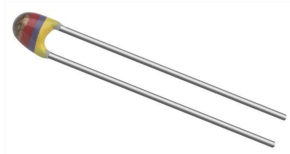
\includegraphics[width=0.3\textwidth]{img/NTC.PNG}
	\caption{Aspecto físico de um termístor NTC.}
	\label{fig:NTCsensor}
\end{figure}

Este sensor possui uma variação de resistência, como mencionado anteriormente. Para a escolha do sensor tem de se verificar na folha de especificações a gama de medições de temperatura que o sensor possibilita e a tolerância do sensor. Em seguida, escolhe-se o valor da resistência para o valor de referência para 25ºC consoante a tolerância do sensor.

Para a integração do sensor num circuito, elabora-se um circuito divisor resistivo com o sensor e a resistência que estabelece o valor de referência para 25ºC, como representa a Figura \ref{fig:NTCmontagem}
\begin{figure}[!htb]
	\centering
	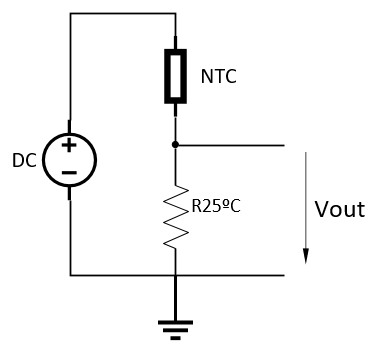
\includegraphics[width=0.3\textwidth]{img/NTCmontagem.PNG}
	\caption{Divisor resistivo com o sensor e a resistência que estabelece o valor de referência para 25ºC.}
	\label{fig:NTCmontagem}
\end{figure}

Para a obtenção de um valor de temperatura exato é necessário obedecer a alguns parâmetros impostos pelo sensor, sendo estes as constantes \(A_1\), \(B_1\) [\(k^{-1}\)], \(C_1\) [\(k^{-2}\)] e \(D_1\) [\(k^{-3}\)]. Após se ter obtido o valor dos parâmetros mencionados recorre-se á equação \ref{eq:Temperatura} na qual serão utilizados os valores dos parâmetros.
\begin{equation}
T [ºC] = \frac{1}{A_1 + B_1*\ln\frac{R}{R_{ref}} + C_1*\ln^2\frac{R}{R_{ref}} + D_1*\ln^3\frac{R}{R_{ref}}}- 273.15
\label{eq:Temperatura}
\end{equation}

É de notar que é subtraído à equação 273.15 para a conversão da temperatura de Kelvin para graus centígrados.

Uma das questões impostas no guião do trabalho de laboratório, é gama total de medição de temperatura que o sensor possibilita. A gama de medição é limitada pela tensão máxima que a entrada analógica da placa de desenvolvimento possibilita, sendo esta 5V DC. 

\newpage

  \section{Circuito implementado}
Nesta secção será descrito o processo de implementação física do projeto, ou seja, a montagem do sensor com a placa de desenvolvimento \textit{Arduino Uno}.

Para a montagem do sensor na placa de desenvolvimento, foi necessário saber qual era a característica do sinal de saída do sensor, para ligar o sensor num porto digital ou analógico. O sensor NTC possui na saída um sinal analógico correspondente a uma variação de tensão. Logo o sensor será ligado a uma entrada analógica com a configuração da Figura \ref{fig:NTCmontagem}. O esquema de ligações do circuito com a placa de desenvolvimento e sensor encontra-se na Figura \ref{fig:CircuitoTotal}.
\begin{figure}[!htb]
    \centering
    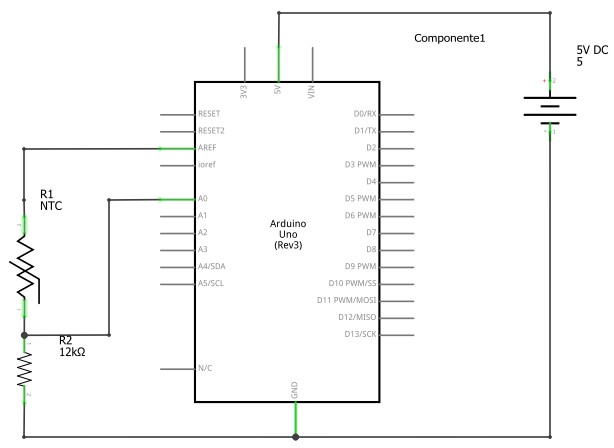
\includegraphics[width=0.7\textwidth]{img/Esquema_de_ligacoes.PNG}
    \caption{Esquema de ligações do sensor na placa de desenvolvimento.}
    \label{fig:CircuitoTotal}
\end{figure}

No código foi definido a resolução da entrada analógica, tendo esta um baud rate de 9600.

A alimentação do circuito é feito internamente, ou seja, é ligado um carregador que fornece 12V DC à placa de desenvolvimento e por meio de um regulador de tensão a tensão é convertida de 12V DC em 5V DC. Na Figura \ref{fig:CircuitoTotal} a alimentação da placa de desenvolvimento está representada por uma fonte de tensão de 5V DC.

No circuito foi colocado uma resistência no divisor de tensão com o sensor NTC de \(12k\Omega\) por lapso, isto porque a resistência devia de ter um valor de \(10k\Omega\), visto o valor referido na folha de especificações do sensor para a resistência uma temperatura de referência de \(25ºC\) ser de \(10k\Omega\). Para ultrapassar este problema, foi colocado no código que o valor da resistência era de \(12k\Omega\), mais concretamente \(12129.0\Omega\), porque o valor da resistência foi medido com um multímetro. Após se ter aplicado este método, foi possível obter valores de temperatura mais precisos.

  \clearpage
  \section{Anexos}
\centering
\center % Center everything on the page
 \vspace*{10cm}
\textsc{\Huge ANEXOS}\\[200cm]

%\section{Código Implementado}
{ \Large \bfseries Código Implementado}\\
\lstinputlisting[language=C]{thermistor.ino}
  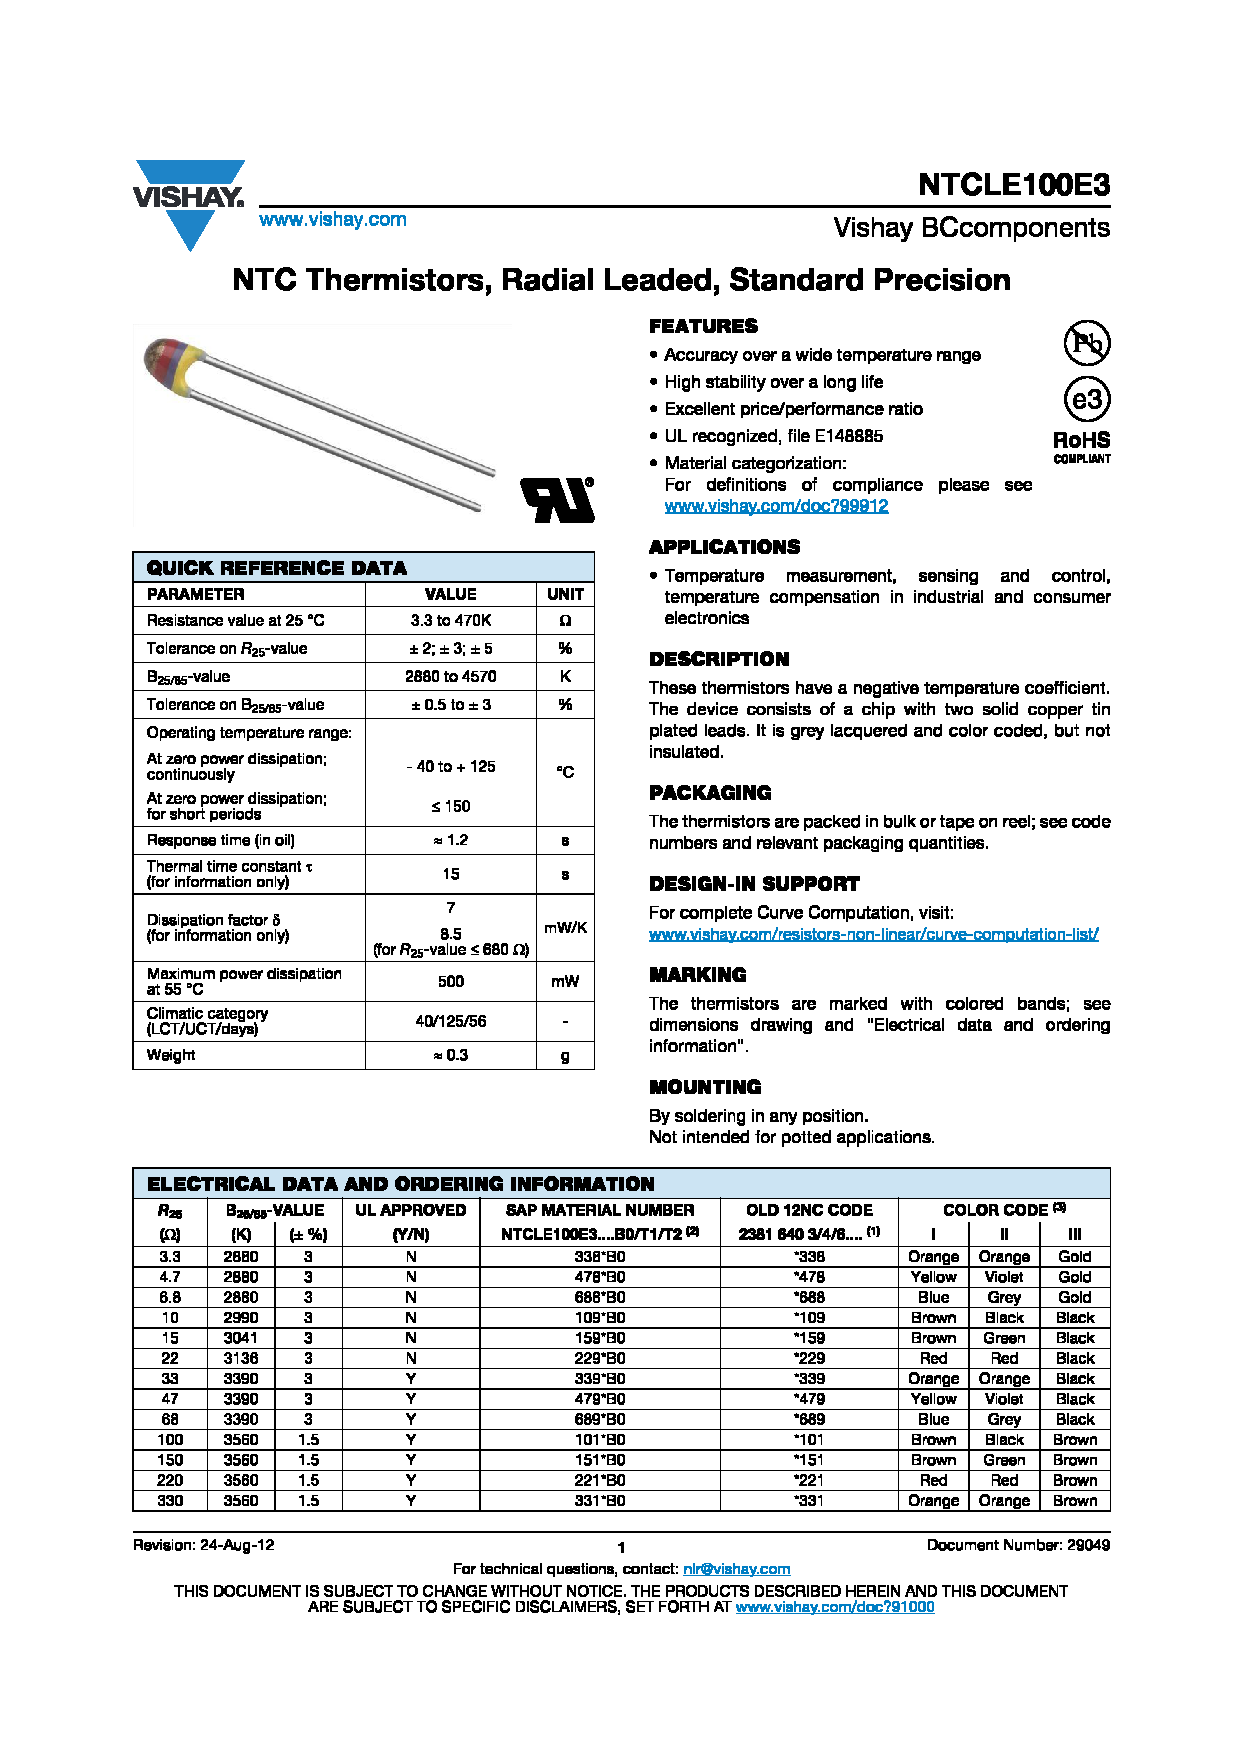
\includepdf[pages={1,2,4},nup=1,landscape=false]{Thermistor_anexos.pdf}

\end{document}
